% Project 1 one-page summary. Build from this folder: pdflatex project1_summary.tex
% Figures: run `python summary/make_figures.py` from the repo root first. They are drawn at
% their printed size, so chart text matches the page's small text.
% Numbers are from step5/bid_calibration_memo.md (21 Oct 2026, after the step-7 re-run),
% real 2026 DKK; EUR at DKK 7.46.
\documentclass[10pt,a4paper]{article}
\usepackage[T1]{fontenc}
\usepackage[utf8]{inputenc}
\usepackage{charter}
\usepackage[a4paper,top=1.5cm,bottom=1.4cm,left=1.8cm,right=1.8cm]{geometry}
\usepackage{graphicx}
\usepackage{booktabs}
\usepackage{array}
\usepackage{xcolor}
\usepackage{microtype}
\usepackage[hidelinks]{hyperref}
\pagestyle{empty}
\setlength{\parindent}{0pt}
\setlength{\parskip}{0pt}
\linespread{1.08}

% ---- Edit your contact line here (e.g. add a LinkedIn URL) ----
\newcommand{\contactline}{\href{https://github.com/fergal567/danish-offshore-cfd-bid-model}{github.com/fergal567/danish-offshore-cfd-bid-model}}

\definecolor{grey}{HTML}{555555}
\newcommand{\head}[1]{\vspace{9pt}{\bfseries #1}\par\vspace{2pt}{\color{grey}\rule{\linewidth}{0.4pt}}\par\vspace{4pt}}
\newcommand{\note}[1]{{\small\color{grey}#1}}

\begin{document}

{\bfseries\Large Reverse-engineering Vattenfall's 2026 Danish offshore wind bids}\par
\vspace{4pt}
{\itshape What do DKK 504/MWh (Nordsøen Midt) and DKK 542/MWh (Hesselø) imply about cost, return and wind?}\par
\vspace{4pt}
{\color{grey} Fergal Israel \quad·\quad Independent analysis from public data \quad·\quad October 2026}\par

\vspace{8pt}
\rule{\linewidth}{0.8pt}\par\vspace{6pt}
Vattenfall's winning prices are 3--6\,\% below what my model needs to break even. They work at a real after-tax return of about 4.5--4.7\,\%, around 1\,pp above Vattenfall's own discount rate for wind, or with 4--6\,\% lower build costs. With 15\,MW turbine costs the return falls to 2.8--3.1\,\%, so the bids look like a bet on 20\,MW turbines.\par
\vspace{6pt}\rule{\linewidth}{0.8pt}\par

\begin{minipage}[t]{0.48\textwidth}
\head{The gap to break-even}
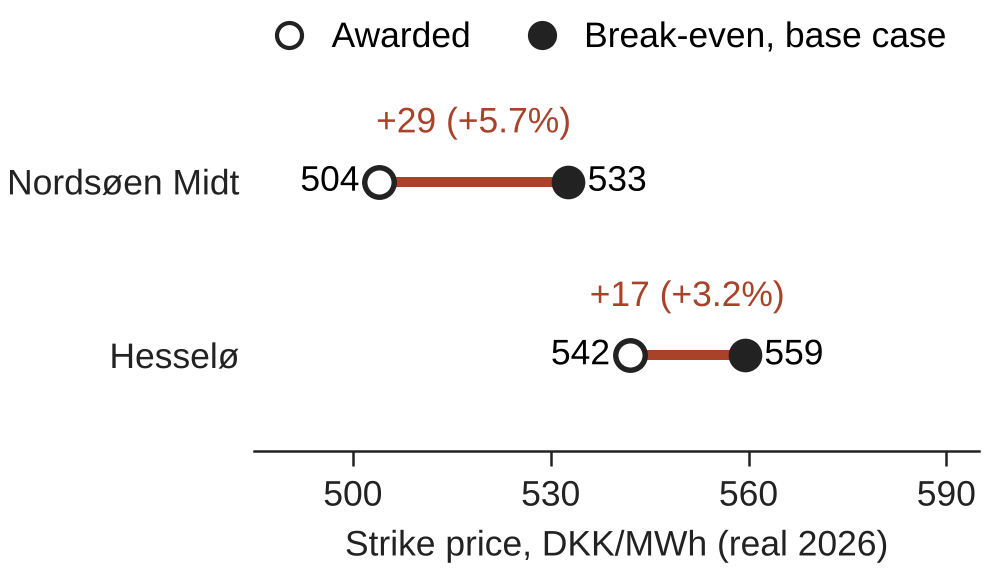
\includegraphics[width=\linewidth]{fig_gap.png}
\end{minipage}\hfill
\begin{minipage}[t]{0.48\textwidth}
\head{Any one of these closes it}
\begin{tabular}{@{}>{\raggedright\arraybackslash}p{0.42\linewidth}>{\raggedleft\arraybackslash}p{0.29\linewidth}>{\raggedleft\arraybackslash}p{0.19\linewidth}@{}}
 & Nordsøen Midt & Hesselø \\
\midrule
Return, real after tax & 4.5\,\% & 4.7\,\% \\[2pt]
Build cost, DKK m/MW & 20.9 & 21.4 \\[2pt]
Wind output & P10 & P10 \\
\bottomrule
\end{tabular}\par
\vspace{5pt}
\note{Base case: 5.0\,\% return, DKK 22.3m/MW (EUR 3.0m), median (P50) output. Vattenfall's 2025 report puts its wind discount rate at about 3.6--5.3\,\% in real terms.}
\end{minipage}

\head{What moves the break-even price}
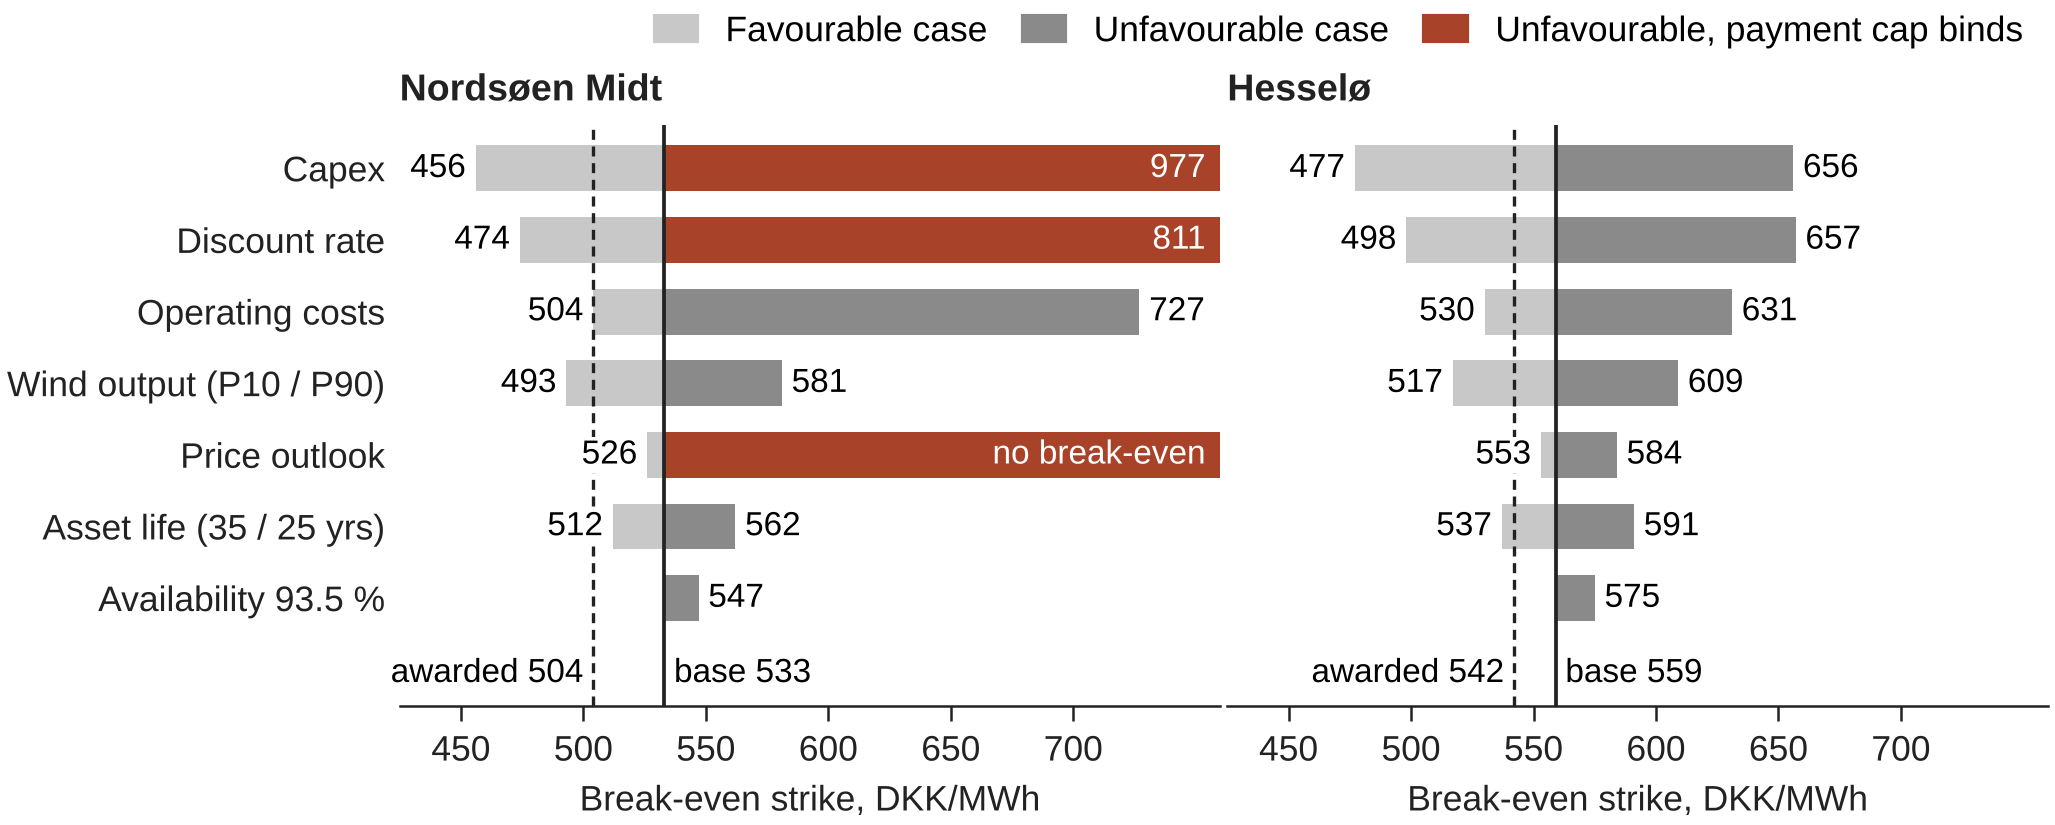
\includegraphics[width=\linewidth]{fig_tornado_summary.png}\par
\vspace{3pt}
\note{One input at a time. Red: the state's cap on CfD payments is used up, so a higher strike adds almost no value.}

\vspace{2pt}
\begin{minipage}[t]{0.48\textwidth}
\head{The bigger risk: the payment cap}
The cap funds an average top-up of DKK 167/MWh at Nordsøen Midt but 313 at Hesselø. In a low-price scenario Nordsøen Midt's cap runs out in July 2047, leaving DKK 5.5bn unpaid. Hesselø never uses more than 76\,\%.
\end{minipage}\hfill
\begin{minipage}[t]{0.48\textwidth}
\head{What it means for the next tender}
Nordsøen Syd (bids due October 2028) has a cap of DKK 6.6bn, about DKK 75/MWh of top-up. Its bidders will have to price the risk of low power prices explicitly. \note{(My interpretation.)}
\end{minipage}

\vfill
{\color{grey}\rule{\linewidth}{0.4pt}}\par\vspace{3pt}
\note{Built from the tender documents, hourly ERA5 wind, Danish power prices and Danish Energy Agency cost and price data, in a monthly 30-year cash-flow model in Python. Contract terms use the Nordsøen Syd documents as a proxy. Not affiliated with Vattenfall, the DEA or Energinet.}\par
\vspace{3pt}
\note{Full memo, code and sources: \contactline}

\end{document}
